\section{Resoconti di verifica ed esiti delle revisioni}

In questa sezione vengono mostrati i valori delle metriche calcolate a termine del periodo di revisione dei requisiti. Saranno mostrati sia i valori che rientrano nel range prestabilito sia quelli che non rientrano, nel secondo caso verranno segnalati come problemi nella parte finale della sezione.

\subsection{Riassunto delle attività di verifica}
Durante il periodo di analisi tutta la documentazione da presentare in ingresso alla revisione dei requisiti è stata sottoposta ad un'analisi meticolosa della struttura del documento, della chiarezza e degli errori ortografici. La verifica di ogni documento è stata svolta da 2 componenti del gruppo per assicurare il minor numero di errori possibili.

\subsection{Risultati delle verifiche tramite analisi}

\subsubsection{Valori dell'indice di Gulpease}

Per ogni documento stilato è stato calcolato l'indice di Gulpease\glo{} in due momenti: al 2021/12/03 e al GG/MM/AAA alla versione 1.0.0 che è stata consegnata per la revisione dei requisiti. I valori sono dati dalla seguente tabella ed il rispettivo grafico con valore sufficiente >40 e valore ottimo >80.

\hphantom{}
\tabulinesep = 2mm % padding
\taburowcolors [1] 2{pari .. dispari} % colori delle righe

\begin{longtabu} to \textwidth {| X[0.2,c m] | X[0.1,c m] | X[0.1,c m] | X[0.1,c m]| X[0.1,c m] | X[0.1,c m] |}
\hline
\rowcolor{header}
\textbf{Data del calcolo} & 
\textbf{Studio di Fattibilità} & 
\textbf{Norme di Progetto} & 
\textbf{Analisi dei Requisiti} & 
\textbf{Piano di Qualifica} & 
\textbf{Piano di Progetto} \\
\hline

\multirow[c]{2}{*}{2020-12-03} & v0.0.8 & v2 & v0.2.4 & v4 & v5 \\
\cline{2-6} 
& 95 & 65 & 61 & 80 & 91 \\ 
\hline
\multirow[c]{2}{*}{data} & v1.0.0 & v1.0.0 & v1.0.0 & v1.0.0 &v1.0.0 \\ 
\cline{2-6} 
& x1 & x2 & x3 & x4 & x5 \\ 
\hline
\end{longtabu}


\newpage
\begin{figure}[htp]
    \centering
    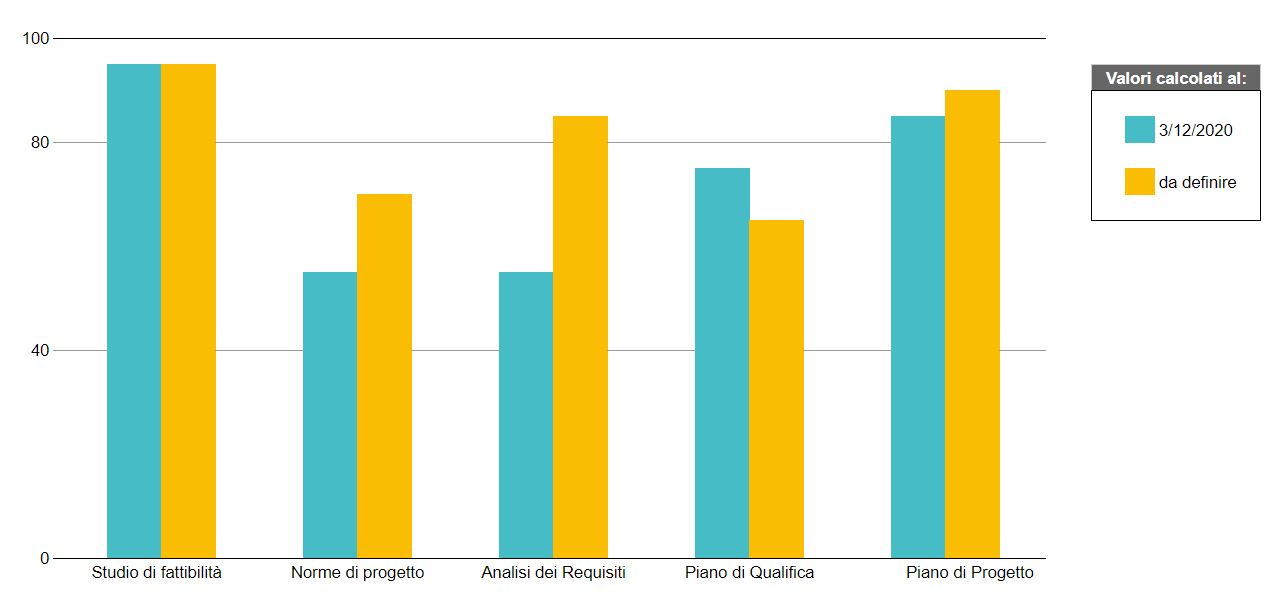
\includegraphics[width=15cm]{GraficoGulpease}
    \caption{Grafico dell'indice di Gulpease}
    \label{fig:img-valori-gulpease}
\end{figure}


\subsubsection{Errori ortografici}

Per quanto riguarda gli errori ortografici, oltre alla revisione fatta dai membri del gruppo, si è utilizzato anche lo spellchecker di Overleaf.


\subsection{Conclusioni}

In conclusione dai valori raggiunti dal grafico e dalla tabella soprastanti, si evince un discreto lavoro di redattori e verificatori.
In particolare sono stati utili il Piano di Qualifica e le Norme di Progetto per avere un punto di riferimento, sia agli analisti nella scrittura dei documenti, sia ai verificatori per controllare con metriche e con parametri oggettivi.

